\documentclass{article}
\usepackage{eecstex}
\usepackage{physics}
\usepackage{pgfplots}

\renewcommand{\thesubsection}{\thesection.\arabic{subsection}}
\renewcommand{\thesubsubsection}{\thesubsection.\alph{subsubsection}}
\renewcommand{\labelenumi}{\arabic{enumi}.}
\newcommand{\F}{\mathcal{F}}
\newcommand{\sinc}{\operatorname{sinc}}
\newcommand{\rect}{\operatorname{rect}}


\title{EE 120 HW 10}
\author{Bryan Ngo}
\date{2021-04-08}

\begin{document}

\maketitle

\section{The Output DTFT of an N-fold Upsampler}

\begin{align}
    y[n] &=
    \begin{cases}
        x\qty[\frac{n}{N}] & n = kN \\
        0 & \text{otherwise}
    \end{cases} \\
    x[n] &= \sum_{k \in \langle p \rangle} X_k e^{j k \omega_0 n}
\end{align}

\subsection{}

\begin{equation}
    y[n] =
    \begin{cases}
        \sum_{k \in \langle pN \rangle} X_k e^{j k \omega_0 \frac{n}{N}} & n = kN \\
        0 & \text{otherwise}
    \end{cases}
\end{equation}
meaning that \(\hat{p} = pN\) and \(\hat{\omega}_0 = \frac{\omega_0}{N}\).

\subsection{}

By the time-scaling property, we can examine all the nonzero terms of one period of the sequence or when \(\bmod(n, N) = 0\),
\begin{align}
    Y_k &= \frac{1}{pN} \sum_{n \in \langle p \rangle} y[nN] e^{-j k \hat{\omega}_0 nN} \\
    &= \frac{1}{pN} \sum_{n \in \langle p \rangle} x[n] e^{-j k \omega_0 n} \\
    &= \frac{1}{N} X_{k \bmod p}
\end{align}
where \(X_k\) is \(p\)-periodic.

\section{A Complex Sampling System}

\subsection{}

Starting with the impulse-train sampled continuous time function
\begin{equation}
    X_p(\omega) = \sum_{n \in \Z} x_c(nT) e^{-j \omega nT} = \frac{1}{T} \sum_{n \in \Z} X_c(\omega - n \omega_s)
\end{equation}
Then, we can plug this into the above equation to get
\begin{equation}
    X_d(e^{j \Omega}) = \frac{1}{T} \sum_{n \in \Z} X_c(\Omega - n \omega_s)
\end{equation}
Our sampling frequency is
\begin{equation}
    \omega_s = 2\cancel{\pi} \frac{\omega_0}{\cancel{\pi}} = 2\omega_0 \implies X_d(e^{j \Omega}) = \frac{1}{T} \sum_{n \in \Z} X_c(\Omega - 2\omega_0 n)
\end{equation}

\begin{center}
    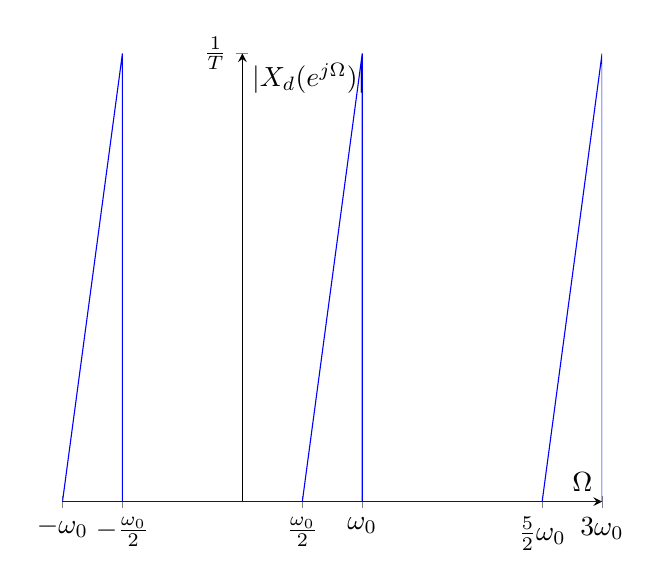
\begin{tikzpicture}
        \begin{axis}[
            xlabel={\(\Omega\)},
            ylabel={\(|X_d(e^{j \Omega})|\)},
            axis lines=middle,
            xtick={-3, -2, 1, 2, 5, 6},
            xticklabels={
                \(-\omega_0\), \(-\frac{\omega_0}{2}\),
                \(\frac{\omega_0}{2}\), \(\omega_0\),
                \(\frac{5}{2}\omega_0\), \(3\omega_0\)
            },
            ytick={1}, yticklabels={\(\frac{1}{T}\)},
        ]
        \addplot[
            color=blue,
        ]
        coordinates{
            (1, 0) (2, 1) (2, 0)
            (5, 0) (6, 1) (6, 0)
            (-3, 0) (-2, 1) (-2, 0)
        };
        \end{axis}
    \end{tikzpicture}
\end{center}

\subsection{}

By inspection, the width of our band-limited signal is \(\frac{\omega_0}{2}\).
\begin{center}
    \begin{tikzpicture}
        \begin{axis}[
            xlabel={\(\Omega\)},
            ylabel={\(H(e^{j \Omega})\)},
            axis lines=middle,
            xmin=0, xmax=3,
            xtick={1, 2},
            xticklabels={
                \(\frac{\omega_0}{2}\), \(\omega_0\),
            },
            ytick={1}, yticklabels={\(T\)},
        ]
        \addplot[
            color=orange,
        ]
        coordinates{
            (1, 0) (1, 1) (2, 1) (2, 0)
        };
        \end{axis}
    \end{tikzpicture}
\end{center}
where we scale by a factor of \(T\) to cancel out the sampling scaling.

\subsection{}

\begin{center}
    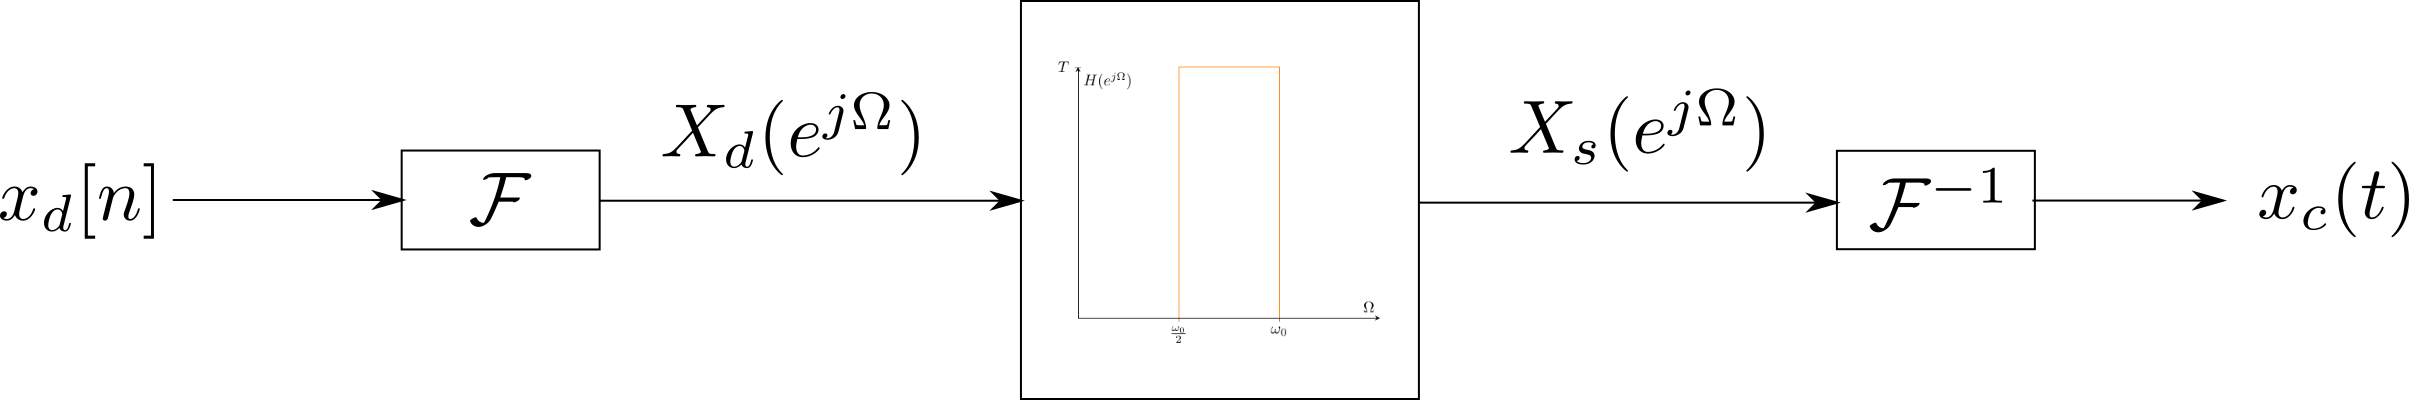
\includegraphics[width=0.8\textwidth]{q2-3.png}
\end{center}

\section{CT Signal for DT System}

\subsection{}

\begin{align}
    h_d[n] &= \frac{1}{2\pi} \int_{-\pi}^\pi \frac{j}{T} \Omega e^{j \Omega n} \, d\Omega = \frac{j}{2\pi T} \int_{-\pi}^\pi \underbrace{\Omega \cos[\Omega n]}_{\text{odd function}} + j\Omega \sin[\Omega n] \, d\Omega \\
    &= -\frac{1}{2 \pi T} \int_{-\pi}^\pi \Omega \sin[\Omega n] \, d\Omega = -\frac{1}{\pi T} \int_0^\pi \Omega \sin[\Omega n] \, d\Omega \\
    &= -\frac{1}{\pi T} \qty(\eval{-\frac{\Omega}{n} \cos[\Omega n]}_0^\pi + \frac{1}{n} \int_0^\pi \cos[\Omega n] \, d\Omega) \\
    &= -\frac{1}{\pi T} \qty(-\frac{\pi}{n} \cos[\pi n] + \frac{1}{n^2} \eval{\sin[\Omega n]}_0^\pi) \\
    &= -\frac{1}{\pi T} \qty(-\frac{\pi}{n} \cos[\pi n] + \frac{1}{n^2} \cancelto{0}{\sin[\pi n]}) = \frac{\cos[\pi n]}{nT} = \frac{(-1)^n}{nT}
\end{align}

\subsection{}

Truncation leaves us with the nonzero values \(\hat{h}_d[-1] = \frac{\alpha}{T}\), \(\hat{h}_d[0] = 0\), and \(\hat{h}_d[1] = -\frac{\alpha}{T}\).
This leaves us with 
\begin{equation}
    \hat{h}_d[n] = \frac{\alpha}{T} (\delta[n + 1] - \delta[n - 1])
\end{equation}
where we take \(\hat{h}_d[0] = 0\) as a degenerate case.
The frequency response is
\begin{align}
    \hat{H}_d(e^{j \Omega}) &= \frac{\alpha}{T} (e^{j \Omega} - e^{-j \Omega}) = \frac{2j \alpha}{T} \sin(\Omega) \\
    &\approx \frac{2j \alpha}{T} \Omega \implies \alpha = \frac{1}{2}
\end{align}
\begin{center}
    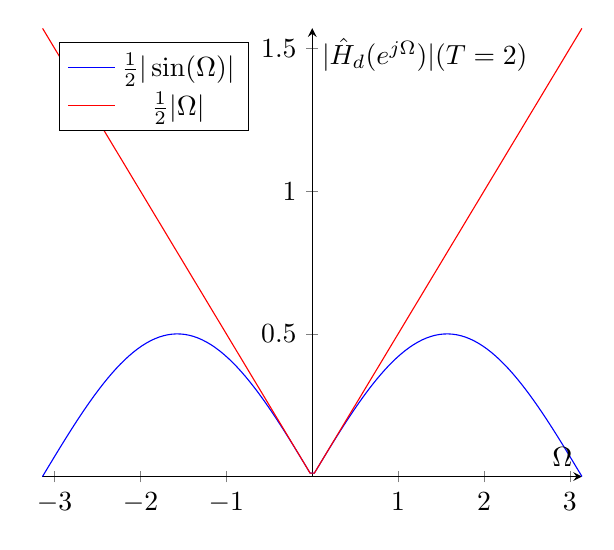
\begin{tikzpicture}
        \begin{axis}[
            xlabel={\(\Omega\)},
            ylabel={\(|\hat{H}_d(e^{j \Omega})| (T = 2)\)},
            axis lines=middle,
            xmin=-pi, xmax=pi,
            legend pos=north west,
        ]
        \addplot[
            color=blue,
            samples=200,
        ]
        {1/2 * abs(sin(deg(x)))};
        \addlegendentry{\(\frac{1}{2} |\sin(\Omega)|\)}
        \addplot[
            color=red,
            samples=200,
        ]
        {1/2 * abs(x)};
        \addlegendentry{\(\frac{1}{2} |\Omega|\)}
        \end{axis}
    \end{tikzpicture}
\end{center}

\subsection{}

\begin{align}
    Y_d(e^{j \omega}) &= \frac{1}{2T} (e^{j \Omega} - e^{-j \Omega}) X_d(e^{j \omega}) \\
    y_d[n] &= \frac{1}{2T} (x[n + 1] - x[n - 1])
\end{align}

\section{2D Sampling}

\begin{equation}
    x_p[n_1, n_2] = x[n_1, n_2] \sum_{k_1 \in \Z} \sum_{k_2 \in \Z} \delta[n_1 - k_1 N_1, n_2 - k_2 N_2]
\end{equation}

\subsection{}

\begin{align}
    X_p(e^{j \omega_1}, e^{j \omega_2}) &= X(e^{j \omega_1}, e^{j \omega_2}) \sum_{k_1 \in \Z} \sum_{k_2 \in \Z} e^{-j (\omega_1 k_1 N_1 + \omega_2 k_2 N_2)} \\
    &= \frac{1}{N_1 N_2} \sum_{k_1 \in \Z} \sum_{k_2 \in \Z} X(e^{j (\omega_1 - k_1 N_1)}, e^{j (\omega_2 - k_2 N_2)})
\end{align}

\subsection{}

We must restrict the bandwidth of \(x[n_1, n_2]\) to half of both \(N_1\) and \(N_2\).

\subsection{}

The impulse response of the filter is a 2D sinc function, namely
\begin{equation}
    h[n_1, n_2] = \frac{1}{4\pi^2} \sinc\qty[\frac{n_1}{2\pi N_1}] \sinc\qty[\frac{n_2}{2\pi N_2}]
\end{equation}
where we scale both by a factor of \(\frac{1}{2\pi}\).

\end{document}
